\cleardoublepage

\chapter{Estado del Arte de la Domótica}
\label{ch:Capitulo2}

Como definición. el término 'domótica' proviene de la unión de las palabras $domus$ (que significa 'casa' en latín) y $-tica$ (de 'automática', palabra en griego que significa ‘que funciona por sí sola’). Se entiende por domótica al conjunto de sistemas que hacen de una vivienda un edificio inteligente, aportando servicios de gestión energética, seguridad, bienestar y comunicación, y que pueden estar integrados por medio de redes interiores y exteriores de comunicación, cableadas o inalámbricas, y cuyo control goza de cierta ubicuidad, desde dentro y fuera del hogar.


Considerar también las conclusiones de sistemas Centralizados y Descentralizados de este artículo.(\url{http://gritosdetecnologia.blogspot.com/2013/04/origen-de-la-domotica.html})

La domótica se remonta a los años 70, uno de los primeros hitos fue el \href{https://es.wikipedia.org/wiki/X10}{protocolo de comunicaciones X-10}~\cite{x10protocolwikipedia} de automatización de dispositivos en la línea eléctrica de un hogar. Con él, se puede utilizar la propia red como canal de comunicaciones mediante ráfagas de pulsos. El ancho de banda de 256 dispositivos simultáneos es una cantidad más que suficiente para interactuar con los dispositivos de un hogar, si calculamos que cada elemento susceptible de ser automatizado como por ejemplo persianas, estufas, enchufes, e interruptores ocupase un espacio de este ancho de banda, seguirían sobrando espacios en un piso de 150 metros cuadrados.

En pleno 2019 pueden adquirirse los dispositivos necesarios para instalar una red X-10 que incluye interruptores, actuadores, sensores, transmisores, interfaces y unidades de control (todos ellos necesarios para obtener el control completo de la red) por precios con rangos entre 20 a 70 euros por cada elemento. Esto supone inversión elevada si se tiene en cuenta un hogar de varias habitaciones. Hay que considerar además ciertas limitaciones como que cada controlador es capaz de manejar un número limitado de dispositivos.

En cuanto a las aplicaciones necesarias para gestionar el sistema, X-10 posee alternativas de código libre para su desarrollo como \href{http://www.minervahome.net/}{Minerva}. También existen interfaces hardware que traducen el protocolo X-10 a APIs de servicios web como el dispositivo \href{http://www.iobridge.com/}{ioBridge} que supuso una disrupción en el ámbito del IoT y la automatización del hogar.

El problema de la solución del X-10 no radica en su protocolo sino en los costes, que generalemente sobrepasan los cientos de euros para las configuraciones mas sencillas. Ademas, esta instalación requiere de un proceso de obra, ya que es necesario empalmar los componente a la red electrica del hogar. En realidad, la opción de usar dispositivos del protocolo X-10 esta comndicionada a que la red electrica del hogar se instalara durante el proceso de edificación comn vistas a utilizar este sistema. De otra forma, sera necesario planificar obras y esto complica la facilidad de crear un prototipo assequeible.

Una década después surgiría el SCE (Sistema de Cableado Estructurado) que permitía el trasporte de datos y voz, esto supuso la aparición del concepto Edificio Inteligente. Sin embargo, esto requiera de una instalación compleja difícilmente viable en edificios ya existentes, como es el caso que ocupa el alcance de este proyecto.

Con la aparición de las redes inalámbricas, y sus posteriores estándares de comunicaci como el WIFI, se popularizaron los sistemas de domótica aplicada directamente sobre los dispositivos, sin tener en cuenta la red eléctrica que los hace funcionar.


\section{Frameworks disponibles para la gestión de IoT para SmartHomes}
\label{ch:Capitulo2.1}

Un planteamiento recurrente en el diseño de una solución basada en software es acelerar el proceso de desarrollo e implementación utilizando un framework. Es una buena idea. Estas herramientas están, en su mayoría, profundamente documentadas para exprimir sus capacidades al máximo, disponen de versionados y revisiones (en mayor o menor medida) que fortalecen tanto su seguridad, robustez, resiliencia e implementación. Poseen una buena abstracción del hardware en el que se ejecutan, sus servicios son modulares, su arquitectura es escalable.  En ocasiones están basados en software libre y/o gratuito, y disponen de una comunidad activa de usuarios a los que poder preguntar dudas. Estas son cualidades muy importantes, mas alla de las capacidades técnicas que cada opción pueda ofrecer.
En el mundo del IoT es impórtate determinar el alcance en conectividad que se desea alcanzar y volumen de datos a tratar. Existen frameworks pensados para interconectar ingentes cantidades de dispositivos en grandes extensiones de terreno y bajo el peso de un abrumador volumen de datos que procesar como es el caso de las SmartCities, o la infraestructura del sector primario y secundario. En algunos casos, el alcance es tan extremo que el concepto de IoT evoluciona a IoE (Internet of Everything) y se requiere la presencia de grandes actores tecnológicos, y sus soluciones, para abarcar estos proyectos, como es el caso del framework IBM BlueMix de IBM, el Cisco Virtualized Packet Core de Cisco, AWS IoT de Amazon o Azure IoT de Miscrosoft, por mencionar algunos ejemplos de este calibre.

Evidentemente, estos frameworks no fueron diseñados pensando en reducidos entornos como los de un hogar, y aunque son compatibles, el tiempo necesario en formación para su uso queda fuera de las capacidades y expectativas de un proyecto de las características que aqui se recoge. Sin embargo, también se dispone de un amplio abanico de opciones a un alcance más acorde a lo esperado de una solución SmartHome.

Existe una serie de criterios que aplicaremos al valorar las opciones de frameworks disponibles, en consonancia con la motivación de este proyecto. Antes de realizar cualquier evaluación sobre las bondades de cada plataforma, es conveniente recordar que en la solución que esperamos crear, se intentara evitar el uso de servicios en la nube o dependencias de APIs externas. Esto responde al objetivo de aislar la suite domótica a desarrollar, de la red de internet, evitando esa dependencia para su operatividad. Por supuesto, no es el objetivo crear una plataforma desconectada, ya que, se espera poder operar de forma remota los dispositivos desde fuera del ámbito de la red local del hogar. Ademas, debera disponer de un licenciamiento de codigo libre y gratuito, en otro caso, estariamos contraviniendo la naturaleza de este proyecto.

FiWare esta catalogada como una plataforma de codigo abierto que agrupan un set de estandares universales para el contexto de gestion de datos~\cite{whatisfiware}. Se sustenta en la ejecución del framework sobre Dockers que pueden ser alojados localmente en maquinas dentro del hogar, y aunque esta solución esta orientada a procesar datos en un contexto mas extenso que una SmartHome, puede aislarse de la red de internet. Limitan la portabilidad de las aplicaciones a aquellas que se catalogen como 'Powered by FIWARE', y aunque ofrecen una interfaz estandar para los componentes que integren la solución, con el objetivo de eliminar el bloqueo del proveedor de componentes, no posee un licenciamiento de codigo libre, por ello sera descartado.

OpenHab es otro nombre que es recomendado frecuentemente en foros y ponencias de IoT, bajo el nombre de 'Open Home Automation Bus', esta plataforma dispone de manuales de instalación para convertir un ordenador en un centro de control de domótica, incluyendo la propia Raspberry Pi con una imagen preconfigurada~\cite{openHabRaspberryPi}. La documentación detalla la definición de un modelo de desarrollo orientado a objetos flexible y escalable, donde las 'things' representan a los dispositivos físicos, que incluyen las propiedades para gestionar sus canales de comunicación a 'items' que representan la capacidades y propiedades de los automatismos del hogar. También se proponen reglas, que definen comportamientos en función de los disparadores asignados por el usuario. De esta forma, puede automatizarse el apagado de las luces de una estancia si en esta no hay individuos. Dispone de un extenso abanico de interfaces, incluyendo un chatbot llamado HABot para controlar la suite domótica con un lenguaje natural escrito, esta función, por ejemplo, ha sido objeto de proyecto en un reciente trabajo de fin de master de la facultad de informática~\cite{eprint49443}. Posee REST API que permite una Inter operatividad con servicios externos o desarrollos propios y soporte para todas las principales plataformas móviles (Android, IOs, Windows) ya que está programado en Java. No se limita tampoco en interoperatividad de buena parte de servicios y stacks de desarrollo existentes, y dispone de una extensa gama de dispositivos compatibles mediante Add-ons, como, por ejemplo, Chromecast o philips Hue, otras soluciones domóticas como ‘Max! Home Solutión’, o protocolos como MQTT o estándares de redes con TCP/UDP o WOL (Wake on LAN) entre otros. De hecho, salvando que su licenciamiento se limita a ser open source, es de lejos, una de las mejores opciones disponibles que cumplen con lo necesario para crear una solución domótica aislada, ya que, no genera dependencias de servicios externos, puede ser operada localmente o de forma remota y dispone de capacidad suficiente en cuanto a soluciones modulares para cubrir los futuros casos de uso que se plantearan.

En el proceso de estudio de diversos frameworks encotnramos otras opciones. En realidad el abanico de soluciones disponibles es muy extenso,

\begin{itemize}
\item thingsboard
\item Pimatic
\item Calaos: Home automation solution and a complete distro
\item Domoticz
\item Home Asistant: Home automation platform running on Python 3
\item OpenMotics : Complete home automation platform
\item Jeedom
\item MisterHouse: Supports X10, voice recognition and several serial devices
\end{itemize}

Ya que uno de los objetivos del proyecto radica en la condición de disponer de una licencia libre, nuestra investigación nos ha llevado a conocer MainFlux. Se cataloga como una plataforma tecnológica de codigo abierto y patente libre con licencia Apache 2..0. Incluso ofrece un dispositivo gateway para soluciones industriales y de computación desarrollada por la misma Linux Foundatión. Esta planteado como PaaS para integrar aplicaciones que interactúan con los dispositivos de la SmartHome mediante un gateway. La plataforma, dispone de una versión gratuita para ser alojado localmente en un Docker o un equipo con SO Linux. Su documentación clarifica que el desarrollo de aplicaciones que conectaran a Mainflux se realizaran a través de protocolos bridging (como HTTP, MQTT,WebSocket, CoAP)~\cite{mainfluxdoc}.



Sin frameworks, aunque supone un mayor esfuerzo, puede orientarse mas concreteamente a nuestros objetivos mas cercanos.

\section{Stack de servicios}
\label{ch:Capitulo2.2}

Habiendo elegido no utilizar un framework concreto, queda a nuestra entera disposición seleccionar bajo que servicios operara nuestra solución domótica. Cualquiera de los frameworks anteriormente listados estaban sujetos a una combinación de servicios que les permitía operar dentro de sus especificaciones. En más de la mitad de ellos, se utilizaban servidores web que permitan gestionar la suite domótica vía web, o a través de una app.

Orientando la selección de los servicios necesarios para la creación de un prototipo, que permita alcanzar los objetivos planteados para este proyecto, surge la necesidad de disponer de un servicio de infraestructura web, que permita gestionar la suite domótica cómodamente desde un dispositivo remoto. Sin entrar en definiciones, nos centraremos en que características que mejor se adapten a las necesidades del proyecto.

Para nuestra estrategia de selección de servicios, empezaremos seleccionando la BBDD que cimentaran el resto de stack. Toda aplicación informática, se sustenta en primera instancia sobre el almacenamiento de datos de manera persistente. En esencia, las BBDD se segmentan en 2 categorías principales según como se relacionan entre si dichos datos. Estos son, BBDD relacionales, o BBDD no relacionales. Además de esta segmentación principal, existen otras características importantes en cuanto a la escalabilidad y diseño de cada modelo. Si consideramos como, humanamente, entendemos los datos necesarios para una suite domótica, una de las primeras impresiones, es que no sabemos con certeza cuantos dispositivos de sensorización o actuadores serán necesarios para cada caso de uso. De hecho, es muy probable que un mismo caso de uso disponga de diferentes combinaciones de dispositivos para alcanzar una solución. Es, sin embargo, bastante obvio que básicamente almacenaremos pocos conceptos primarios, los principales son, ubicaciones, dispositivos en las ubicaciones y medidas y/o acciones de los dispositivos.

Podría parecer que hablamos de una relación de objetos entre sí, y que un modelo de BBDD relacional es la mejor opción, pero si consideramos que, cada entrada almacenada tendrá una estructura distinta, hace que no sea una opción tan ideal.

Pensemos, por ejemplo, que utilizando una BBDD SQL se planifica un conjunto de tablas relacionadas entre sí. Sera necesaria una tabla que contenga las ubicaciones y se relacione con otra tabla que definan a los dispositivos. Esto establece una relación 1:N donde múltiples dispositivos pueden existir para una estancia, pero nunca en varias a la vez. De cada dispositivo existirá una nueva relación 1:N de medidas. Lo cual deja un esquema semejante al de la figura siguiente:


\begin{figure}[hbt!]
\centering
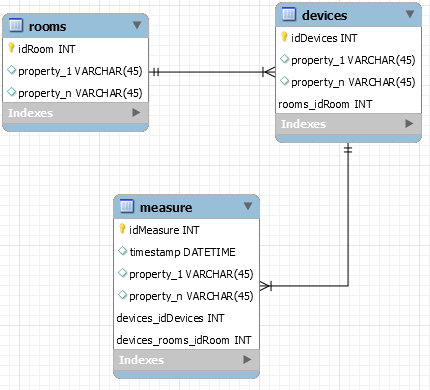
\includegraphics[height=2.5in]{figures/SQLSchemaExample_1.jpg}
\end{figure}

Sin embargo, existen algunos problemas graves de diseño de esta idea, en primer lugar, los dispositivos no pueden ser una propiedad de una estancia. Son objetos relacionados, pero no existe una transitividad dura entre ellos. Un dispositivo puede cambiar de estancia en un momento dado, y aun asi, seguir existiendo medidas en fechas concretas de ese dispositivo para una habitación en la cual, dicho dispositivo ya no está relacionado. Otro posible escenario es la desaparición de una estancia (como resultado de fusionar 2 estancias en una al derribar una pared). Para mantener una integridad lógica y persistente a lo largo del tiempo. Toda medida deberá tener un campo que determine en que ubicación fue tomada.
no hay transitividad dura entre room y device, lo cual hace que sean independientes entre sí.


\begin{figure}[hbt!]
\centering
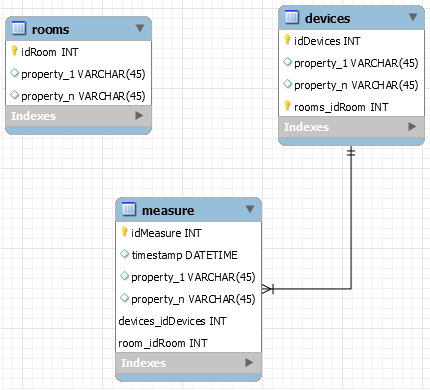
\includegraphics[height=2.5in]{figures/SQLSchemaExample_2.jpg}
\end{figure}

Con esto aún tendríamos que enfrentar un problema adicional, el número de columnas que definen las propiedades de una tabla. El ejemplo más claro es la tabla de medidas. Una medida, efectuada por un sensor será definida por su identificador y la fecha en la que se realizó, ahora bien, según la naturaleza del dispositivo, se obtendrán disantos tiempos de medida. Un sensor combinado de temperatura y humedad nos dará dos magnitudes de medición, un sensor de ruido almacenará un valor de decibelios, una luz define su medida por su estado de actividad (encendido o apagado), aunque por otra parte podría indicar el consumo eléctrico, o propiedades adicionales como intensidad de luz, o incluso color. Es cierto que, para un actuador, como lo es un emisor de luz, no realiza medidas como tal, y sus correspondientes estados de actividad podrían ser más adecuados definirlos como propiedades del dispositivo y no como medidas. Podríamos separar las medidas de los estados en tablas distintas, pero igualmente llegaríamos al problema del número de campos necesarios en una tabla. Valor que por otra parte es muy difícil de prever en base a la extensa gama de dispositivos existentes. Esto puede solucionarse de manera sencilla con 2 estrategias. Incluir una gran cantidad de columnas en previsión de los distritos tipos de medidas existentes, dejando que las medidas posean un valor nulo para los campos no utilizados en función de la relación de su sensor, o bien, unificar todos los campos en un único valor de cadena de caracteres que almacene un dato estructurado, como es el caso de los JSON. Esta última opción, sería la más deseable tanto por sencillez de implementación como facilidad de procesamiento. Lo que dejaría un esquema semejante a este:

\begin{figure}[hbt!]
\centering
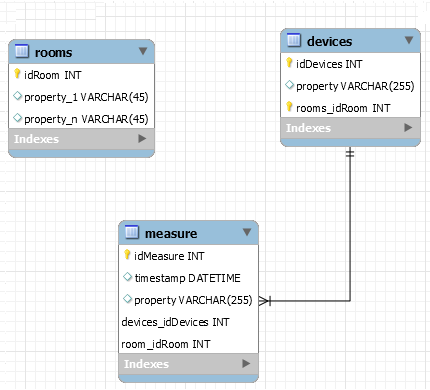
\includegraphics[height=2.5in]{figures/SQLSchemaExample_3.png}
\end{figure}

Una preocupación que agrava la perspectiva de usar una BBDD relacional es que, en este punto del proyecto, es su escalabilidad horizontal. Si bien las tablas pueden crecer a un gran número de registros, no se prevé almacenar datos con vistas a largo plazo, la mayoría de los valores almacenados serán efímeros en tiempo de utilidad, almenarlos responde solo a la necesidad de obtener comparativas en plazo de tiempo relativamente cortos, como horas, dias, y posiblemente semanas. Mas alla de este rango estos datos no tienen una utilidad real y pueden ser condensados en medias para utilizarse en resúmenes. Por otro lado, disponer de flexibilidad a la hora de configurar la extensión de propiedades de un objeto de la BBDD es uno de los puntos fuertes de una BBDD no relacional.

En primer lugar, es necesario que se trate de un servidor web ligero en ejecución. En segundo lougar no es necesario que tenga gran capacidad de atender a muchos usuarios simultanemente.

MEAN vs LAMP



\section{Protocolos de comunicación y selección}
\label{ch:Capitulo2.3}


El protocolo MQTT
El protocolo AMBIENTAL
